\documentclass{article} 

\usepackage{polski}              
\usepackage[utf8]{inputenc}
\usepackage{graphicx}
\usepackage{float}
\usepackage{amsmath}
\usepackage{hyperref}

\author{Rafał Wiensko \\Wojciech Zygmuntowicz}
\title{Sprawozdanie na temat lawin}
\begin{document}
\maketitle

\newpage
 
\section{Wstęp}
	\subsection{Cel projektu}

		Celem projektu było zbadanie praw zachodzących przy rozchodzeniu się lawin śnieżnych, jednak prawdą jest, że te same zasady obowiązują także przy rozchodzeniu się piasku na kopczykach, 
		pożarów w lasach, epidemii chorób w miastach, a także wielu innych niezwiązanych z samymi lawinami przypadkach.  W tym sprawozdaniu opisano w jaki sposób zbadano zachowanie się lawin
		oraz przedstawiono wyniki i porównano je z oczekiwanym rezultatem.

	\subsection{Model teoretyczny}

		W celu symulacji spadania lawiny skorzystano z tzw. automatu komórkowego, tj. podzielono powierzchnię góry na $n^{2}$ powierzchni $P_{i j}$. Każda powierzchnia posiada pewną średnią 
		wysokość $h_{i j}$. Następnym krokiem jest obliczenie lokalnego spadku $S_{i j}$, wg następującej zasady: 
			

			\[ S_{i j} = h_1 + h_2 - h_3 - h_4 \]
			
			
		%	\begin{figure}[h]
		%		\begin{center}
		%			\includegraphics [bb = 0 0 340 318, scale=0.5] {Slope_ij.png}
		%		\end{center}
		%	\end{figure}
		
		Dla każdej automaty definiujemy lokalny spadek progowy, powyżej którego pozwalamy, aby przemieścił się śnieg. Jeżeli zostanie on przekroczony następuje lokalne zsunięcie się śniegu, czyli:
		
			\[ h_1 \rightarrow h_1 - 1 \]
			\[ h_2 \rightarrow h_2 - 1 \]
			\[ h_3 \rightarrow h_3 + 1 \]						
			\[ h_4 \rightarrow h_4 + 1 \]
			
		Dodatkowo potrzebujemy mechanizmu, który sprawi że będzie się pojawiał nowy śnieg, definiujemy dwa mechanizmy sypania śniegu: zachowawczy i niezachowawczy. Sypanie zachowawcze polega
		na zwiększaniu wysokości losowo wybranej powierzchni $h_{i j}$ o jednostkę. Z drugiej strony mechanizm niezachowawczy polega na zwiększaniu losowo wybranego lokalnego spadku $S_{i j}$, 
		czyli na zwiększeniu wysokości całego rzędu, lub kolumny od losowo wybranej współrzędnej do górnego krańca powierzchni o jednostkę.
		\newline

		Potrzeba także zdefiniować zachowanie się automaty na jej krawędziach, z tego też powodu wprowadza się tzw. otwarte i zamknięte warunki brzegowe. Otwarte warunki brzegowe pozwalają na 
		wysypywanie się śniegu poza obszar automaty, zamknięte sprawiają, że śnieg nie może się z niego wydostać. 
						
	\subsection{Samoorganizujące się systemy krytyczne}
		
		W przypadku ciągłego dosypywania śniegu będą powstawać coraz to nowe lawiny. Na początku tylko lokalne, jednak z czasem będą zajmować coraz to większy obszar automaty. Warto w tym momencie 
		wprowadzić kolejną wielkość, jaką jest średni spadek automaty: 

			\[ <S> = \frac{ \sum_{i, j}^{} S_{i j} }{n^2} \] 

		W sytuacji krytycznej jedno sypnięcie (mowa tu o mechaniźmie sypania śniegu) spowoduje globalną lawinę. Okazuje się jednak, że gdyby śnieg sypać dostatecznie długo, to $<S>$ nigdy nie przekroczy
		pewnej granicznej wartości, co więcej $<S>$ nigdy też nie spadnie poniżej pewnej wartości, będzie do niej dążył. Jest to pewnego rodzaju równowaga w jakiej utrzymuje się układ. Stan ten nazywany jest atraktorem. Wartość graniczna jest niezależna od sposobu, 
		w jaki sypiemy śnieg. Zależy zaś w pewnym stopniu od rozmiaru automaty, a także od tego, czy użyto otwartych, czy zamkniętych warunków brzegowych. Ponieważ zamknięte warunki brzegowe
		wymuszają zerowanie się lokalnego spadu na granicy automaty (aby śnieg nie mógł się przemieścić poza automatę), średni spadek $<S>$ będzie w tym przypadku mniejszy.
		
	\subsection{Prawo potęgowe}
		
\section{Wyniki}

	Automatę zaimplementowano w języku skryptowym ruby, wyniki zaś zostały narysowane w formie wykresów w programie gnuplot. Na początku porównano zależności średniego nachylenia w zależności od liczby sypań śniegu $<S>(t)$ dla różnych rozmiarów automaty, symulację odbyto przy spadku progowym równym 7, niezachowawczym sypaniu śniegu oraz przy otwartych warunkach brzegowych, odpowiednio dla: n = 10, n = 20 i n = 40. Wykres zamieszono poniżej: 
		\begin{figure}[h]
			\begin{center}
				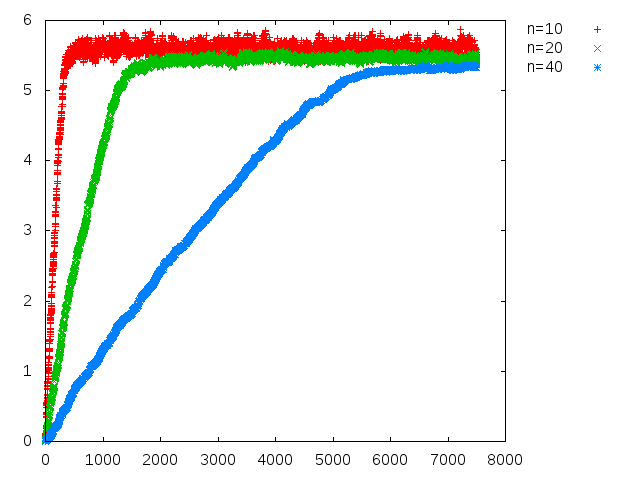
\includegraphics [bb = 0 0 340 318, scale=0.5] {average_slope_threshold_7.png}
			\end{center}
		\end{figure}
\newpage
	Jak widać średnie nachylenie $<S>$ niezależnie od rozmiaru automaty zmierza do jednej wartości, którą jest $S_{gr} = 5.4$. Okazuje się także, że wartość ta nie zmienia się też dla lawin o większej liczbie swobody, niż 1. Choć wydawać się może, że analizowanie czegoś takiego, jak lawiny w liczbie wymiarów większej niż 3 jest bezcelowe, to należy pamiętać, że wyniki symulacji są dużo bardziej ogólne niż tylko dla lawin i obejmują także rozchodzenie się np. chorób w społeczeństwie, gdzie liczba stopni swobody może być większa niż 2. 

	Kolejna symulacja została przeprowadzona w celu 

	

\section{Podsumowanie}

	Samoorganizujące się systemy krytyczne są to układy, w których atraktorem jest punkt krytyczny. Za pomocą implementacji automaty komórkowej pokazano,  że przy odpowiednich zasadach lawiny śnieżne są właśnie samoorganizującymi się systemami krytycznymi i będą dążyć do stanu krytycznego. Zaskakujące jest, że podobne własności przejawiają także pożary lasów, epidemie oraz trzęsienia ziemi. Jest to kolejny przypadek w fizyce, kiedy rozwiązując specyficzny problem otrzymano odpowiedź na zachowanie się całej klasy układów.

\section{Bibliografia}

	\href {http://www.hiskp.uni-bonn.de/uploads/media/sandpiles.pdf}{Daniel Shmeier, Oliver Freyermuth - Sandpiles - Self Organized Critical Systems}
	
\end{document}
